\section{Aims and Objectives}

The aim of this project is to develop and deploy a prototype IoT architecture with the purpose of collecting data relevant to the health of the Griffith footbridge. This involves implementing the first five layers of the architecture which consist of the coding layer, perception layer, network layer, middle-ware layer and application layer. This deployment will be achieved through the testing and implementation of two prototypes.

The first prototype is designed for testing the software and the first three layers of the IoT architecture. Two Arduino MKRWAN 1300 devices will be used, one acting as the LoRa node (layer one and two) and the other acting as a pseudo LoRaWAN gateway (layer three). The first MKRWAN 1300 is equipped with an ADXL335 3-axis accelerometer and is placed on a metal beam. The beam is vibrated along the z-axis and the device samples the acceleration. The device finds the maximum frequency peak and maximum acceleration and transmits the data via a LoRa packet. The second device receives the LoRa packet and logs the data via a serial connection. A python program is used to establish serial connection with the devices and log the output to a text file. Another python program is then used to plot the serial output data using matplot library pyplot. The high level system diagram in figure \ref{Proto1HLSD} presents the desired implementation of this prototype. 

\begin{figure}[h]
	\centering
	\caption{Prototype 1 High Level System Diagram}
	\label{Proto1HLSD}
	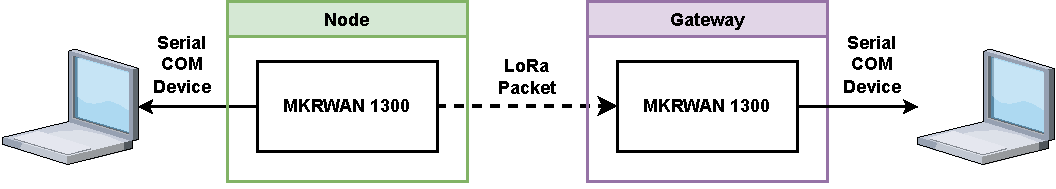
\includegraphics[scale=0.8]{Sections/Introduction/Prototype-1-High-Level.drawio.pdf}
\end{figure}

The aims of prototype 1 will be satisfied once the following objectives are met.

\begin{enumerate}
	\item{Verify that the two MKRWAN devices are capable of communicating over the LoRaWAN protocol}
	\item{Integrate an accelerometer onto the node and write software that samples and discretizes the raw acceleration values}
	\item{Write software to compute the FFT of these discrete values and find the peak frequency}
	\item{Write software to log and plot the raw acceleration from the node}
	\item{Send and receive the maximum acceleration and peak frequency from the node to the gateway}
	\item{Write software to log and plot the maximum acceleration and peak frequency from the gateway}
	\item{Test the maximum range of LoRa packets between the node and gateway}
\end{enumerate}

The second prototype is designed for testing the software, PCB, enclosure and first five layers of the IoT architecture. The two MKRWAN 1300 devices are now both nodes and are implemented onto a custom designed PCB. This PCB is enclosed in a custom 3D printed enclosure and sits behind the guard rail of the Griffith foot bridge. The two nodes sample the maximum frequency and maximum acceleration of the bridge and transmit this data via LoRa packets to a Wisgate Edge Lite 2 LoRaWAN gateway. This gateway uploads the data via WIFI or Ethernet to the TNN cloud which acts as the middle-ware layer. --- APPLICATION LAYER WHAT IS THE IMPLEMENTATION --- Figure \ref{Proto2HLSD}
displays the high level system diagram for the second prototype. 

\begin{figure}[h] 
	\centering
	\caption{Prototype 2 High Level System Diagram}
	\label{Proto2HLSD}
	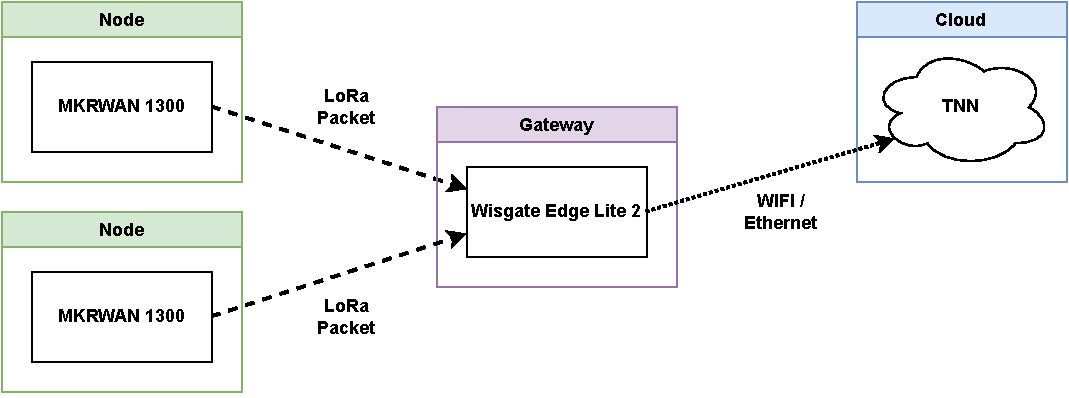
\includegraphics[scale=0.8]{Sections/Introduction/Prototype-2-High-Level.drawio.pdf}
\end{figure}

--- ADD TO PROTO 2 OBJECTIVES ONCE I COMPLETE TESTING ---
The aims of prototype 2 will be satisfied once the following objectives are met.

\begin{enumerate}
	\item{Design, fabricate and test a custom PCB to replace the breadboard from prototype 1}
	\item{Design and fabricate an enclosure to be placed behind the rail of the Griffith footbridge}
	\item{Configure both MKRWAN devices as nodes and establish a LoRaWAN connection to the gateway with a network connection to the cloud}
	\item{Create a cloud application to log LoRa packets from the nodes}
	\item{Verify software and range capabilities through system integration testing on the bridge}
\end{enumerate}


